\usepackage{wrapfig}
\begin{document}
\textbf{Størrelse:} \\
Da Danmark har gode forhold for vindenergi, kommer det ikke som en overraskelse, at der er stor fokus på udvikling indenfor området, og især hvad gælder vindmøller. Ifølge energiforliget for år 2020, så skal halvdelen af Danmarks energiforbrug være dækket igennem vindenergi. Dette vil bl.a. ske ved at reducere antallet af vindmøller installeret på land og i stedet fokusere på havvindmøller. %(http://www.windpower.org/da/energipolitik_og_planlaegning/energiforliget_og_2020.html)
Et andet tiltag for at øge energiudbyttet fra vindmøller er ved at optimere selve vindmøllerne. Herved kan der ses på vindmøllernes vingelængde, hvilket bestemmer det bestrøgne areal af den vind, som møllerne påvirkes af. Formlen for det bestrøgne areal er lig formlen for et cirkelareal:
\begin{equation}
A = \pi * r^2
\end{equation}
Det bestrøgne areal har indflydelse på den effekt, som vindmøllerne yder, hvilket gør vingelængden på vindmøllerne vigtig for det givne udbytte af energi. Jo større vingemålene bliver, des større effekt, men det stiller også større krav til f.eks. møllens generator og konstruktion, så den ikke bliver revet i stykker. Igennem de sidste tredive år har europæiske regeringer finansieret eksperimentelle vindturbiner til videre udvikling. Ved år 2001 blev der opsat havvindmøller med en diameter for det bestrøgne areal på 112 meter, hvilket kunne generere en effekt på 4,5 MW. Ti år senere i år 2011 var diameteren for det bestrøgne areal steget til 160 meter, hvorved møllerne kunne generere 8 MW.
\begin{figure}[H]
\centering
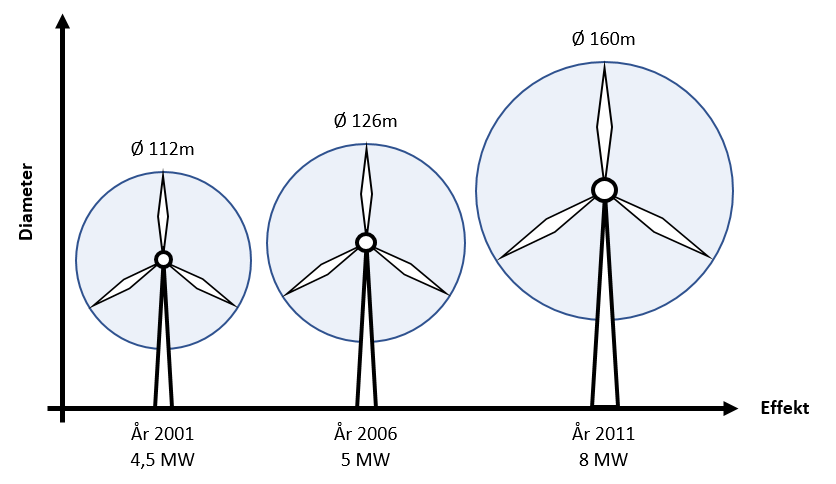
\includegraphics[scale=0.85]{Billeder/Vindmoelle_udvikling}
\caption{Udviklingen af størrelse og effekt for havvindmøller sponsoreret af regeringer i Europa}
\end{figure}

Private virksomheder er begyndt at følge med og overhale de eksperimentelle havvindmøller, hvor Vestas A/S opførte havvindmøller med en diameter på 164 meter med en effekt på 7 MW i år 2011.

Oversigt over virksomheders største vindmøller 2011: %(https://books.google.dk/books?id=mEtBN5L1Q2UC&printsec=frontcover&dq=isbn:9789814364935&hl=da&as_brr=3&cd=1&source=gbs_api#v=onepage&q&f=false)
\begin{table}[H]
\centering
\begin{tabular}{l|l}
Vestas \ \ \ \ & \ \ \ \ $Ø164 m$ med $7 MW$ \\
Nordex \ \ \ \ & \ \ \ \ $Ø150 m$ med $6 MW$ \\
Bard \ \ \ \ & \ \ \ \ $Ø122 m$ med $6,5 MW$ \\
Alstom \ \ \ \ & \ \ \ \ $Ø150 m$ med $6 MW$ \\
NPS \ \ \ \ & \ \ \ \ $Ø175 m$ med $8 MW$
\end{tabular}
\end{table}
Udviklingen indenfor vindmølleindustrien er fortsat i gang, hvor der forsøges at producere mere effektive vindmøller end de eksisterende. Så sent som i december 2016 blev der prøvekørt prototypen på en ny $8 MW$ vindturbine produceret gennem et samarbejde mellem Vestas Wind Systems A/S og Mitsubishi Heavy Industries (MHI). Denne prototypes platform er blevet modificeret, så det er muligt at generere en effekt på op til $9 MW$ under de rigtige forhold. \\
MHI Vestas forklarer, at turbinerne kan indsættes i eksisterende $8 MW$ havvindmøller, hvilket gør dem i stand til at opnå en effekt på de $9 MW$ ved samme rotorareal. Dette medfører, at der mindskes udgifter for opbygningen af vindmølleparker, bl.a. i form af ændringen på allerede opførte havvindmølleparker, da turbinerne kan udskiftes i stedet for selve møllerne. Derudover skal der færre vindmøller til for at leve op til effektkravet omkring havvindmølleparker, hvilket gør produktionen af parkerne billigere. %(http://www.mhivestasoffshore.com/new-24-hour-record/)
Under testkørslen af turbinen, blev der genereret $215.999,1 kWh$ over 24 timer, hvilket er tilsvarende den energi, som skal benyttes til at forsyne omkring 20.000 husstande. Ud fra dette slog prototypen verdensrekord for energi produceret. %(https://ing.dk/artikel/mhi-vestas-presser-sin-8-mw-moelle-paa-9-mw-192758)
\newpage
\textbf{Støj:} \\
Vindmøller er maskiner, hvilket gør, at de udsender støj. Denne støj kan have indflydelse på beboere i nærheden af møllerne, og derfor er der opsat regulativer for, hvor meget vindmøller må støje. For landbaserede vindmøller er støjgrænsen for møllerne inddelt i to kategorier alt efter, om møllerne er placeret i et åbent miljø, eller om de står nær bebyggelse. Ved opbygningen af en ny vindmølle skal lyden fra omkringliggende møller medregnes, så den totale sum ikke overskrider støjgrænsen. Målingen for støj foretages ved en afstand af 15 meter fra det mest støjende punkt omkring møllen ved to forskellige vindhastigheder, henholdsvis 6m/s og 8m/s. Ved en vindhastighed på 6m/s, hvor landbaserede vindmøller i et åbent miljø har en støjgrænse på 42dB, mens vindmøller nær bebyggelse har en støjgrænse på 37dB. Ved en højere vindhastighed på 8m/s er grænsen opsat til 44dB ved et åbent miljø og 39dB nær bebyggelse. For alle landbaserede vindmøller ved begge vindhastigheder må den lavfrekvense støj ikke overstige 20dB. Lavfrekvens støj har en frekvens på mellem 10-160Hz. %(http://journals.sagepub.com/doi/pdf/10.1260/0263-0923.31.4.239)
For målingerne skal det dog siges, at målingerne for vindmøllerne kan være upræcise, da det er umuligt at sortere baggrundsstøjen fra omgivelserne fra. \\
\begin{wrapfigure}{l}{8cm}
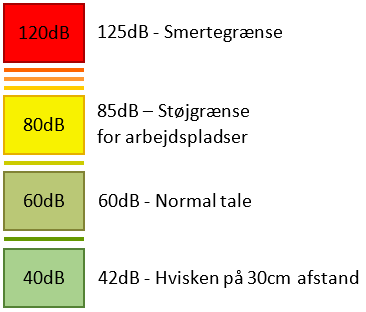
\includegraphics[scale=1]{Billeder/Stoejgraenser}
\end{wrapfigure}
\\
Ved støjgrænserne mellem 37-44dB er der ikke fare for direkte høreskader. En lydstyrke på 44dB er tilsvarende en hvisken på en afstand af 30cm, så at være udsat for denne lydstyrke vil ikke have direkte konsekvenser for ens hørelse. De lavfrekvente lyde er ikke så almindelige i omgivelserne hvilket gør, at de kan virke mere forstyrrende for hørelsen. Grænseværdien på 20dB svarer til en 3,6MW vindmølle på 1800 meters afstand, så færden tættere på møllerne kan forekomme irritabelt. %(http://dkvind.dk/fakta/P7.pdf)
\\

For tiden bliver der investeret i store landbaserede vindmøller. I perioden mellem 2004 og til 2015 er der blevet opført 465 produktionsmøller i Danmark med en kapacitet på mellem 2MW til 3,6MW, hvilket har været hovedparten af nye landbaserede vindmøller. %(http://www.dkvind.dk/html/nogletal/pdf/statusnotat_0216.pdf)
Netop for denne størrelse af landbaserede vindmøller er der blevet foretaget målinger og beregninger for at se, om de holder sig indenfor regulativerne omkring støjniveau. Bilag X % (http://vbn.aau.dk/files/227978180/2012_Pedersen_et_al_LF_Stratford_u_A.pdf)
viser, hvordan forskellige vindmøller indenfor størrelsesordenen 2MW til 3,6MW holder sig under grænsen på 44dB for almindelig støj ved et åbent miljø, men det kan ikke måles præcist nok, hvorvidt de holder sig under grænsen for lavfrekvens støj, så dette skal derfor beregnes. Tabel X angiver de beregnede værdier indenfor de danske regulativer, hvad angår lavfrekvens støj indendørs ved husstande: \\
\begin{table}[H]
\centering
\begin{tabular}{|r|r|r|r|r|r|r|} \hline
Frekvens (Hz) & 10 & 16 & 31,5 & 63 & 125 & 160 \\ \hline
dB & -2 & -2 & 5,5 & 12,5 & 17 & 21,5 \\ \hline
\end{tabular}
\end{table}

Ud fra dette kan det ses, at den lavfrekvente støj ikke overskrider støjgrænsen på de 20dB før enden af det lavfrekvente spekter på 160dB nås. %(http://vbn.aau.dk/files/227978180/2012_Pedersen_et_al_LF_Stratford_u_A.pdf )
\\
Udledningen af støj fra vindmøller kan inddeles i to kategorier; mekanisk og aerodynamisk. Den mekaniske støj stammer fra de bevægelige mekaniske dele ved selve vindmøllen f.eks. generator, gearboks og køleblæser. Denne type støj kommer i form af tonal støj, hvilket kan forekomme mere irritabelt for hørelsen, da det adskiller sig fra naturlige toner. Aerodynamisk støj forekommer hovedsageligt, når vindmøllevingerne bevæger sig gennem luften. Herved dannes der luftstrømme, som fremkalder en karakteristisk susende lyd. Den aerodynamiske støj følger en bredbåndslyd, hvilket forekommer ved frekvenser på højere end 100Hz. %(http://search.proquest.com/docview/1549924292/fulltext/6FE1E10AADF44220PQ/7?accountid=8144)
\end{document}